% fs-04-Bayes.tex

\documentclass[xcolor=dvipsnames]{beamer}

\usepackage{graphicx}
\usepackage{wrapfig}
\usepackage{colortbl}
\usepackage{alltt}
\definecolor{myblue}{rgb}{0.8,0.85,1}

\mode<presentation>
{
  \usetheme{Warsaw}
  \setbeamercovered{transparent}
}
% \usecolortheme[named=OliveGreen]{structure}
\setbeamertemplate{navigation symbols}{} 
\setbeamertemplate{blocks}[rounded][shadow=true] 

\newif\ifBCITCourse
\BCITCoursetrue
% \BCITCoursefalse
\newif\ifWhichCourse
\WhichCoursetrue
% \WhichCoursefalse
\ifBCITCourse
\ifWhichCourse
\newcommand{\CourseName}{Statistics for Food Technology}
\newcommand{\CourseNumber}{MATH 2441}
\newcommand{\CourseInst}{BCIT}
\else
\newcommand{\CourseName}{Calculus for Geomatics}
\newcommand{\CourseNumber}{MATH 2511}
\newcommand{\CourseInst}{BCIT}
\fi
\else
\newcommand{\CourseName}{Philosophy and Literature}
\newcommand{\CourseNumber}{PHIL 375}
\newcommand{\CourseInst}{UBC}
\fi

\title{Bayes and Conditional Probability}
\subtitle{{\CourseNumber}, BCIT}

\author{\CourseName}

\date{January 30, 2017}

% \begin{figure}[h]
% 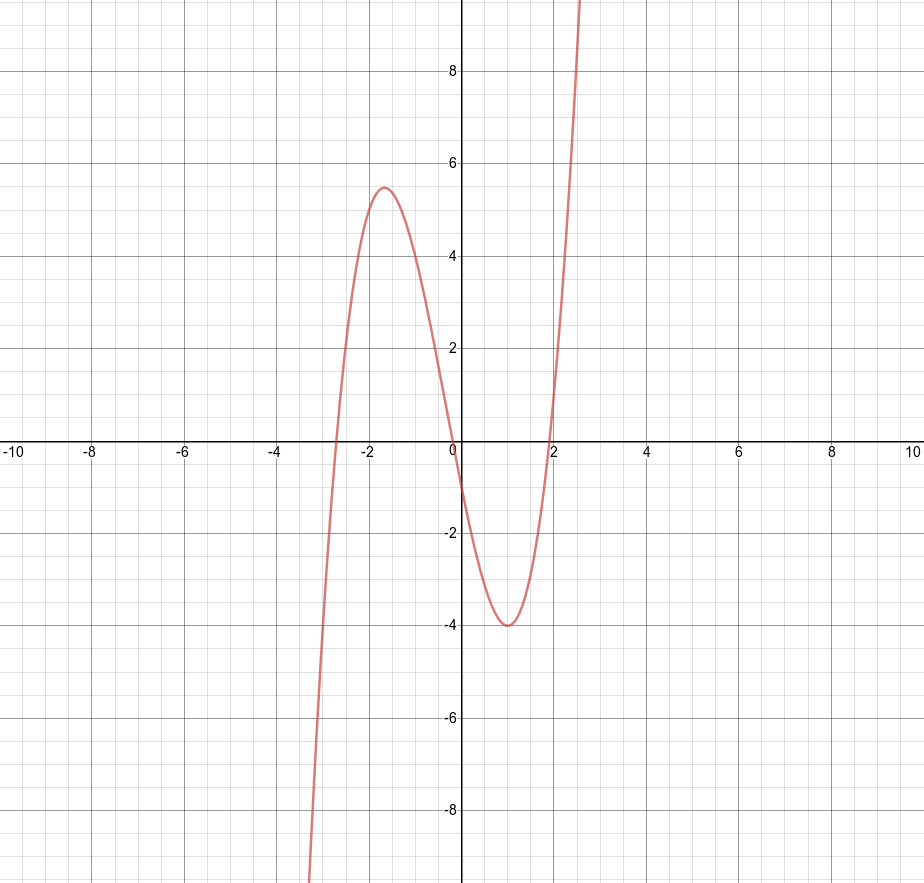
\includegraphics[scale=.3]{./diagrams/extrema1.png}
% \end{figure}

% Command             10pt    11pt    12pt
% \tiny               5       6       6
% \scriptsize         7       8       8
% \footnotesize       8       9       10
% \small              9       10      10.95
% \normalsize         10      10.95   12

\begin{document}

\begin{frame}
  \titlepage
\end{frame}

\begin{frame}
  \frametitle{xkcd on Bayes' Formula}
\begin{figure}[h]
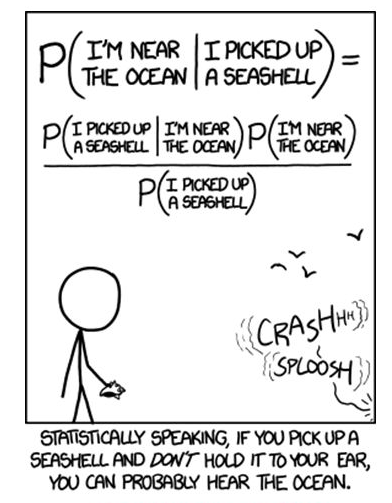
\includegraphics[scale=.5]{./diagrams/xkcd_bayes1.png}
\end{figure}
\end{frame}

\begin{frame}
  \frametitle{Conditional Probability}
Let's remember what conditional probability means.
% \begin{equation}
%   \label{eq:ohyeweeb}
%   P(B|A)=\frac{P(B\cap{}A}{P(A)}
% \end{equation}
\begin{figure}[h]
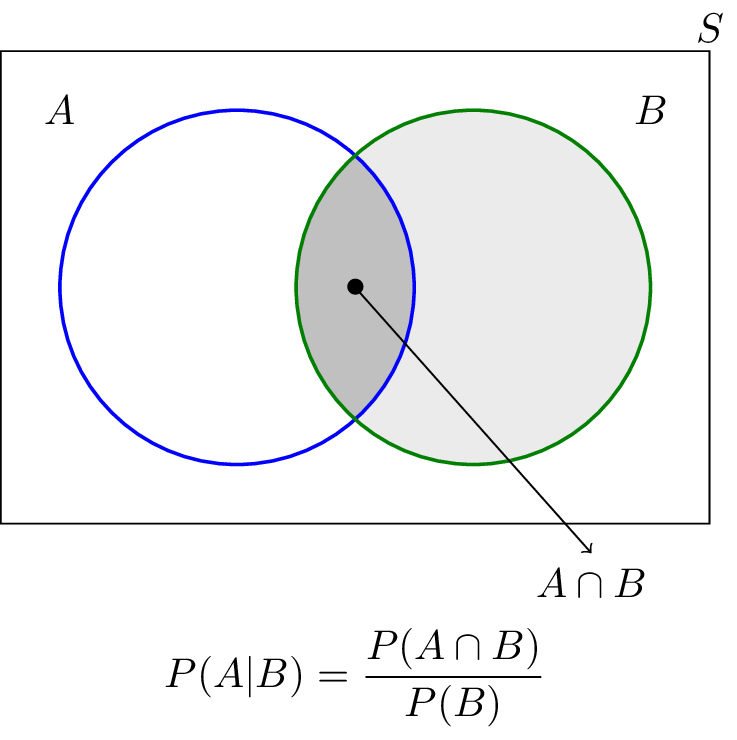
\includegraphics[scale=.25]{./diagrams/conditional_b.png}
\end{figure}
\end{frame}

\begin{frame}
  \frametitle{Multiplication Rule}
  Remember the thief who wants to crack the four-digit PIN of a bank
  card. Let $A$ be the event that she successfully cracks the PIN. If
  $A_{1}$ is the event that she succeeds on her first attempt (and so
  on for $A_{2}$ and $A_{3}$), then
\begin{equation}
  \label{eq:ragheidu}
  P(A)=P(A_{1}\cup{}A_{2}\cup{}A_{3})=P(A_{1})+P(A_{2})+P(A_{3})=0.003
\end{equation}
because $A_{1},A_{2},A_{3}$ are disjoint. We are assuming that her
attempts happen \alert{without replacement}. Therefore,
$A_{1},A_{2},A_{3}$ are not independent, and the correct application of
the multiplication rule is
\begin{equation}
  \label{eq:mohghunu}
  P(A)=1-P(\urcorner{}A)=\notag
\end{equation}
\begin{equation}
  \label{eq:yoobaegh}
  1-P(\urcorner{}A_{1})\cdot{}P(\urcorner{}A_{2}|\urcorner{}A_{1})\cdot{}P(\urcorner{}A_{3}|\urcorner{}A_{1}\cap{}\urcorner{}A_{2})=0.003
\end{equation}
\end{frame}

\begin{frame}
  \frametitle{Law of Total Probability}
It is often easier to calculate conditional probabilities than
unconditional probabilities. To express one by the other use the
\alert{law of total probability},
\begin{equation}
  \label{eq:aefengah}
  P(A)=P(A|B)P(B)+P(A|\urcorner{}B)P(\urcorner{}B)
\end{equation}
This formula also applies when you split up $B$ into three or more
disjoint subsets that exhaust $B$. It follows from set theory.

\bigskip

\textbf{Example: }Suppose that two factories supply light bulbs to the
market. Factory X's bulbs work for over 5000 hours in 99\% of cases,
whereas factory Y's bulbs work for over 5000 hours in 95\% of cases.
It is known that factory X supplies 60\% of the total bulbs available.
What is the chance that a purchased bulb will work for longer than
5000 hours?
% Now we should be able to answer the question from last week: How many
% four digit numbers are there with no repeating digits?
\end{frame}

\begin{frame}
  \frametitle{Law of Total Probability}
\textbf{Example: }Suppose that two factories supply light bulbs to the
market. Factory X's bulbs work for over 5000 hours in 99\% of cases,
whereas factory Y's bulbs work for over 5000 hours in 95\% of cases.
It is known that factory X supplies 60\% of the total bulbs available.
What is the chance that a purchased bulb will work for longer than
5000 hours?

\bigskip

Let $X$ be the event that the light bulb is from factory X. Let $F$ be
the event that the bulb will work for longer than
5000 hours. Then
\begin{equation}
  \label{eq:uwahiamo}
  P(F)=P(F|X)P(X)+P(F|\urcorner{}X)P(\urcorner{}X)=\notag
\end{equation}
\begin{equation}
  \label{eq:siecafoo}
  0.99\cdot{}0.60+0.95\cdot{}0.40=0.974
\end{equation}
\end{frame}

\begin{frame}
  \frametitle{Law of Total Probability Exercises I}
What is the probability that the second card in a conventional
deck of cards is an ace?
\end{frame}

\begin{frame}
  \frametitle{Law of Total Probability Exercises II}
Suppose we have two hats: one has 4 red balls and 7 green balls,
the other has 11 red and 5 green. We toss an unfair coin (60/40 for
heads), if heads, pick a random ball from the first hat, if tails from
the second. What is the probability of getting a red ball?
\end{frame}

\begin{frame}
  \frametitle{Law of Total Probability Exercises III}
You have three bags that each contain 100 marbles:
\begin{itemize}
\item Bag 1 has 75 red and 25 blue marbles
\item Bag 2 has 60 red and 40 blue marbles
\item Bag 3 has 45 red and 55 blue marbles
\end{itemize}
I choose one of the bags at random and then pick a marble from the
chosen bag, also at random. What is the probability that the chosen
marble is red?
\end{frame}

\begin{frame}
  \frametitle{Some Interesting Cases}
  A group of police officers have breathalyzers displaying false
  drunkenness in 5\% of the cases in which the driver is sober.
  However, the breathalyzers never fail to detect a truly drunk
  person. One in a thousand drivers is driving drunk. Suppose the
  police officers then stop a driver at random, and force the driver
  to take a breathalyzer test. It indicates that the driver is drunk.
  We assume you don't know anything else about him or her. How high is
  the probability he or she really is drunk?
\end{frame}

\begin{frame}
  \frametitle{Some Interesting Cases}
  A room is full of engineers and lawyers (most of them are lawyers,
  90\%). The probability that an engineer enjoyed physics in school is
  80\%. The probability that a lawyer enjoyed physics in school is
  30\%. You ask someone in the room whether they enjoyed physics, and
  the answer is yes. Should you bet that this person is a lawyer, or
  should you bet that she is an engineer?
\end{frame}

\begin{frame}
  \frametitle{Some Interesting Cases}
You have a million food items, of which 1 in 1000 is contaminated. You
have a contamination test with a 2\% false positive rate and a 0.5\%
false negative rate. A food item tests positive for contamination.
What is the probability that it is contaminated?
\end{frame}

\begin{frame}
  \frametitle{Some Interesting Cases}
  In a city of 1 million inhabitants let there be 100 terrorists and
  999,900 non-terrorists. To simplify the example, it is assumed that
  all people present in the city are inhabitants. Thus, the base rate
  probability of a randomly selected inhabitant of the city being a
  terrorist is 0.0001, and the base rate probability of that same
  inhabitant being a non-terrorist is 0.9999. In an attempt to catch
  the terrorists, the city installs an alarm system with a
  surveillance camera and automatic facial recognition software.

The software has two failure rates of 1\%:
\begin{itemize}
\item The false negative rate: If the camera scans a terrorist, a bell
  will ring 99\% of the time, and it will fail to ring 1\% of the
  time.
\item The false positive rate: If the camera scans a non-terrorist, a
  bell will not ring 99\% of the time, but it will ring 1\% of the
  time.
\end{itemize}

Suppose now that an inhabitant triggers the alarm. What is the chance
that the person is a terrorist?
\end{frame}

\begin{frame}
  \frametitle{Bayes' Formula}
Consider the definition of conditional probability,
\begin{equation}
  \label{eq:ohyeweeb}
  P(B|A)=\frac{P(B\cap{}A)}{P(A)}
\end{equation}
Now notice that $P(B\cap{}A)=P(A\cap{}B)=P(B)P(A|B)$. That means that
\begin{equation}
  \label{eq:maifiepu}
  P(B|A)=\frac{P(B)P(A|B)}{P(A)}
\end{equation}
By the law of total probability we can replace the denominator to give
us \alert{Bayes' Formula}
\begin{equation}
  \label{eq:ohrughai}
  P(B|A)=\frac{P(B)P(A|B)}{P(A|B)P(B)+P(A|\urcorner{}B)P(\urcorner{}B)}
\end{equation}
\end{frame}

\begin{frame}
  \frametitle{Base Rate Fallacy Diagram}
\begin{figure}[h]
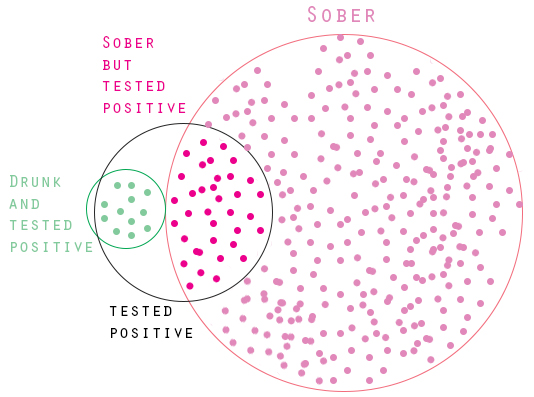
\includegraphics[scale=.4]{./diagrams/Detect-drunk-driving.jpg}
\end{figure}
\end{frame}

\begin{frame}
  \frametitle{Base Rate Fallacy Example}
  Let 100 out of 100,000 people have a disease. The test for this
  disease has a 5\% \alert{false positive} rate and a 5\% \alert{false
    negative} rate. If you test positive for this disease, what is
  your probability of actually having the disease. Consider the
  following \alert{contingency table} and then apply Bayes'
  formula.
\begin{figure}[h]
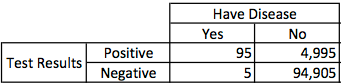
\includegraphics[scale=.7]{./diagrams/baserate3.png}
\end{figure}
\end{frame}

\begin{frame}
  \frametitle{Contingency Tables}
\begin{figure}[h]
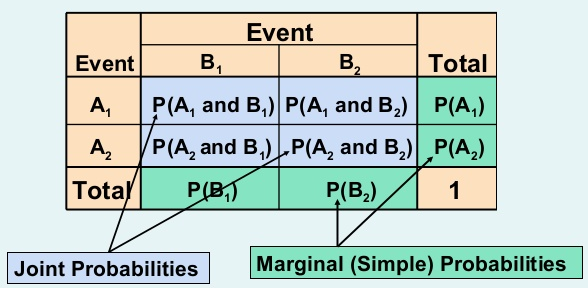
\includegraphics[scale=.5]{./diagrams/contingency1.png}
\end{figure}
\end{frame}

\begin{frame}
  \frametitle{Prison and Plea}
Here is a contingency table:
\begin{tabular}{|l|c|c|}\hline
  & Guilty Plea & Plea of Not Guilty \\ \hline
  Sentenced to Prison & 392 & 58 \\ \hline
  Not Sentenced to Prison & 564 & 14 \\ \hline
\end{tabular}
\end{frame}

\begin{frame}
  \frametitle{Prison and Plea}
Answer the following questions:
\begin{enumerate}
\item<1-> Find the probability of a randomly selected subject being
  sentenced to prison.
\item<2-> Find the probability of being sentenced to prison, given
  that the subject entered a plea of guilty.
\item<3-> Find the probability of being sentenced to prison, given
  that the subject entered a plea of not guilty.
\item<4-> Find the probability of a randomly selected subject being
  sentenced to prison or entering a plea of guilty.
\item<5-> If two subjects are randomly selected, find the probability
  that they were both sentenced to prison.
\item<6-> If two subjects are randomly selected, find the probability
  that they both entered pleas of not guilty.
\item<7-> Find the probability of a randomly selected subject being
  entering a plea of not guilty or not being sentenced to prison.
\item<8-> Find the probability of a randomly selected subject being
  sentenced to prison and entering a plea of guilty.
\item<9-> Find the probability of a randomly selected subject not being
  sentenced to prison and not entering a plea of guilty.
\end{enumerate}
\end{frame}

\begin{frame}
  \frametitle{Exercises I}
% J.V. Uspensky, Introduction to Mathematical Probability, p40
Three urns contain respectively 1 white and 2 black balls; 3 white and
1 black ball; 2 white and 3 black balls. One ball is taken from each
urn. What is the probability that among the balls drawn there are 2
white and 1 black?
\end{frame}

\begin{frame}
  \frametitle{Exercises I}
% J.V. Uspensky, Introduction to Mathematical Probability, p40
Three urns contain respectively 1 white and 2 black balls; 3 white and
1 black ball; 2 white and 3 black balls. One ball is taken from each
urn. What is the probability that among the balls drawn there are 2
white and 1 black? Answer: $23/60$
\end{frame}

\begin{frame}
  \frametitle{Exercises II}
% Devore and Peck, Statistics, p247
A student has a box containing 25 computer disks, of which 15 are
blank and 10 are not. She randomly selects disks one by one and
examines each one, terminating the process only when she finds a blank
disk. What is the probability that she must examine at least two disks?
\end{frame}

\begin{frame}
  \frametitle{Exercises II}
% Devore and Peck, Statistics, p247
A student has a box containing 25 computer disks, of which 15 are
blank and 10 are not. She randomly selects disks one by one and
examines each one, terminating the process only when she finds a blank
disk. What is the probability that she must examine at least two
disks? Answer: 40\%
\end{frame}

\begin{frame}
  \frametitle{Exercises III}
% Devore and Peck, Statistics, p247
There are five faculty members in a certain academic department. These
individuals have 3, 6, 7, 10, and 14 years of teaching experience,
respectively. Two of these individuals are randomly selected to serve
on a committee. What is the probability that they have at least 15
years of teaching experience?
\end{frame}

\begin{frame}
  \frametitle{Exercises III}
% Devore and Peck, Statistics, p247
There are five faculty members in a certain academic department. These
individuals have 3, 6, 7, 10, and 14 years of teaching experience,
respectively. Two of these individuals are randomly selected to serve
on a committee. What is the probability that they have at least 15
years of teaching experience? Answer: 60\%
\end{frame}

\begin{frame}
  \frametitle{Exercises IV}
% Devore and Peck, Statistics, p249
Suppose three cards are selected from a well-mixed deck without
replacement. 
\begin{enumerate}
\item<1-> What is the probability that all three are hearts?
\item<2-> What is the probability that all three are from the same
  suit?
\item<3-> If five cards are dealt from a randomized deck, determine
  the probability that they are all hearts.
\end{enumerate}
\end{frame}

\begin{frame}
  \frametitle{Exercises IV}
% Devore and Peck, Statistics, p249
Suppose three cards are selected from a well-mixed deck without
replacement. 
\begin{enumerate}
\item What is the probability that all three are hearts? Answer: $1.29$\%
\item What is the probability that all three are from the same
  suit? Answer: $5.18$\%
\item If five cards are dealt from a randomized deck, determine
  the probability that they are all hearts. Answer: $0.0495$\%
\end{enumerate}
\end{frame}

\begin{frame}
  \frametitle{Exercises V}
% Devore and Peck, Statistics, p250
  A tennis coach has brought out 12 tubes of Penn balls and 8 tubes of
  Wilson balls for his class. If 5 tubes are randomly selected, what
  is the probability that all 5 are of the same brand?
\end{frame}

\begin{frame}
  \frametitle{Exercises V}
% Devore and Peck, Statistics, p250
  A tennis coach has brought out 12 tubes of Penn balls and 8 tubes of
  Wilson balls for his class. If 5 tubes are randomly selected, what
  is the probability that all 5 are of the same brand? Answer: $5.47$\%
\end{frame}

\begin{frame}
  \frametitle{Exercises VI}
\begin{figure}[h]
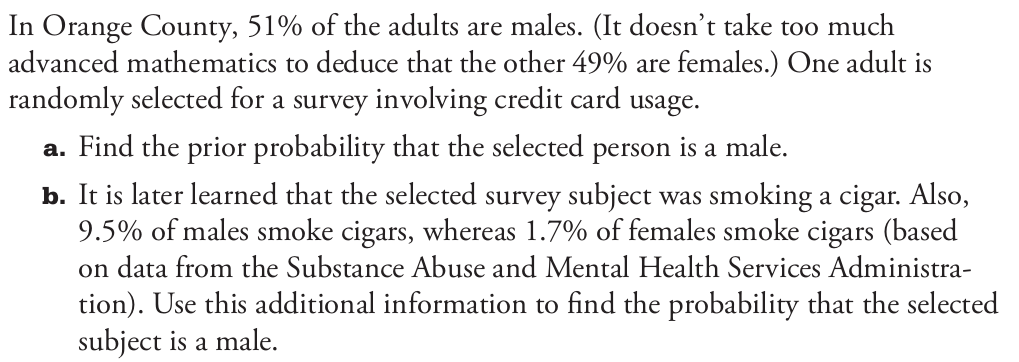
\includegraphics[scale=.32]{./diagrams/triola_bayes1.png}
\end{figure}
\end{frame}

\begin{frame}
  \frametitle{Exercises VI}
\begin{figure}[h]
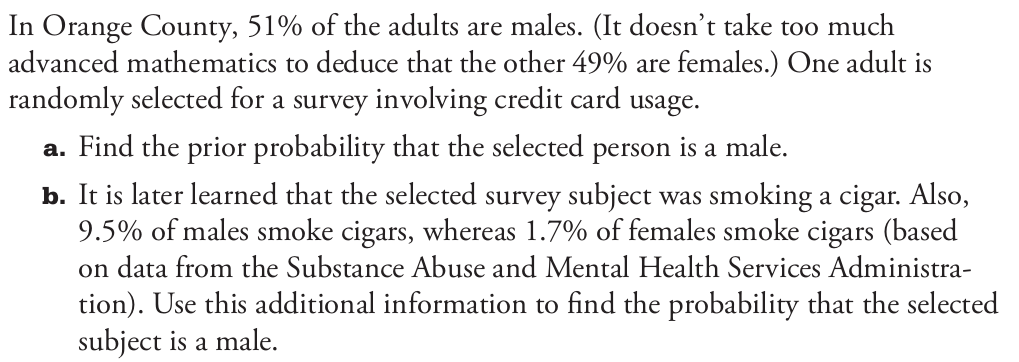
\includegraphics[scale=.32]{./diagrams/triola_bayes1.png}
\end{figure}
Answer: (a.) $51$\% (b.) $85.3$\%
\end{frame}

\begin{frame}
  \frametitle{Exercises VII}
\begin{figure}[h]
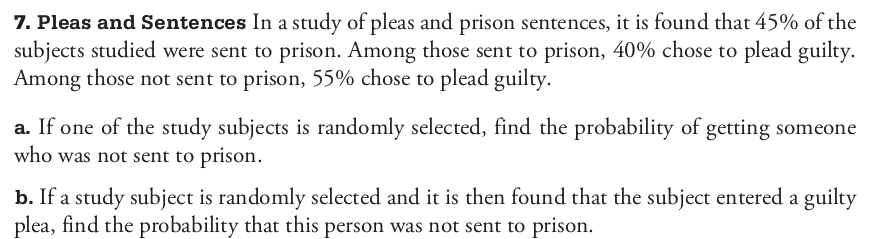
\includegraphics[scale=.36]{./diagrams/triola_bayes2.png}
\end{figure}
\end{frame}

\begin{frame}
  \frametitle{Exercises VII}
\begin{figure}[h]
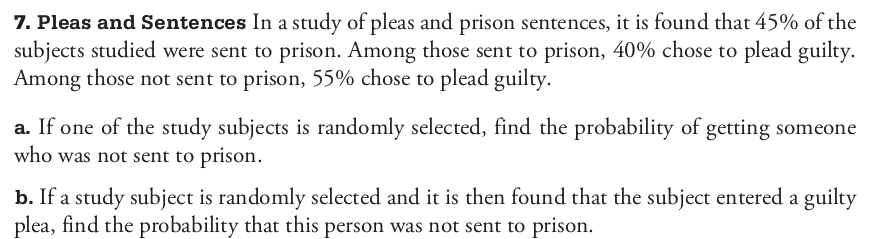
\includegraphics[scale=.36]{./diagrams/triola_bayes2.png}
\end{figure}
Answer: (a.) $55$\% (b.) $62.7$\%
\end{frame}

\begin{frame}
  \frametitle{Exercises VIII}
\begin{figure}[h]
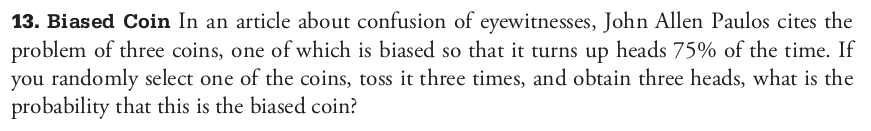
\includegraphics[scale=.36]{./diagrams/triola_bayes3.png}
\end{figure}
\end{frame}

\begin{frame}
  \frametitle{Exercises VIII}
\begin{figure}[h]
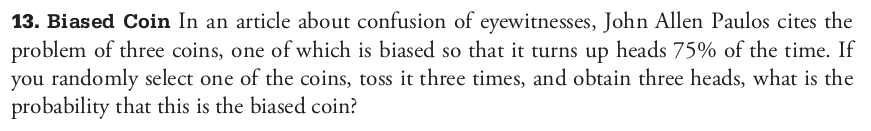
\includegraphics[scale=.36]{./diagrams/triola_bayes3.png}
\end{figure}
Answer: $62.8$\%
\end{frame}

\begin{frame}
  \frametitle{End of Lesson}
Next Lesson: Uniform and Binomial Distribution
\end{frame}

\end{document}
